% HOW TO: a chapter starts with \chapter{...}. It always begins a new page and
% is numbered automatically ("CHAPTER I").
\chapter{Introduction}

This chapter is a working example of every element the template supports. Each
element is preceded by a one-line \verb|% HOW TO:| comment in the source file,
so the pattern can be copied without first learning the machinery behind it.
Delete the whole file once your own first chapter is written; nothing else
depends on it.

Write ordinary paragraphs like this one. The class takes care of margins, line
spacing, the running header and the page number, and it applies the Graduate
School's rules whether or not you remember them. Nothing in this file sets a
length, a font size, or a spacing command, and nothing in your own chapters
needs to either. If you find yourself reaching for a spacing command, the
formatting is probably already correct and the instinct is worth resisting.

The one habit the template cannot supply is order. Introduce a figure or a
table in the text before it appears, keep the numbering in the order you
mention things, and let the class place them.

% HOW TO: first-level subheading (numbered 1.1).
\section{First-level Subheadings}

A first-level subheading opens a major division of the chapter. The heading
levels below it are styled distinctly from one another, so a reader can tell
depth by eye as well as by number, and they are tagged as a real heading
hierarchy so that a screen reader can navigate between them.

Levels should be used in order, without skipping. A subsection inside a
chapter with no intervening section is legal LaTeX and a genuine accessibility
defect, because it leaves a gap in the outline that assistive technology
reports as a structural error.

% HOW TO: second-level subheading (numbered 1.1.1).
\subsection{Second-level subheadings}

Text under a second-level subheading. Most chapters will not need more than
three levels; the remaining two exist for the occasions that do, and are shown
here so that their appearance is known in advance rather than discovered
during a formatting review.

% HOW TO: third-level subheading (unnumbered by default).
\subsubsection{Third-level subheadings}

Third-level subheadings are unnumbered by default, on the view that a
four-part decimal number is harder to read than the words it precedes. If your
committee wants them numbered, that is a one-line change in the class.

% HOW TO: fourth-level subheading.
\paragraph{Fourth-level subheadings}

Fourth-level subheadings are set in the body face, distinguished only by the
space around them. They mark a turn in the argument rather than a new topic.

% HOW TO: fifth-level subheading; it runs into the paragraph that follows.
\subparagraph{Fifth-level subheadings} Please do not use fifth level subheadings. 
Fourth is probably excessive too. This is not a rule of the graduate school, 
but everyone will think you are a goober. If absolutely necessary, the fifth level 
runs into the paragraph it introduces, which is the conventional way to label a 
definition or an aside without spending a whole line on it. Anything finer than this 
is better handled with a list or a plain sentence.

\section{Lists}
% HOW TO: bulleted list.
Lists are tagged as real lists, so the number of items and the boundary
between them are announced correctly. Use them for genuinely parallel
material, not to break up prose:

\begin{itemize}
  \item an unnumbered item, for things with no inherent order,
  \item and a second unnumbered item.
\end{itemize}

% HOW TO: numbered list.
Numbered lists carry the additional claim that the order matters, which is
worth honouring:

\begin{enumerate}
  \item A numbered item.
  \item A second numbered item.
\end{enumerate}

\section{Figures, Tables and Equations}
\subsection{Figures}

% HOW TO: a figure needs four things -- alt={...} describing it in one or two
% sentences for a screen reader, a \caption, a \label, and a \ref to it in the
% text BEFORE the figure appears.
%
% CAPTION VARIANTS, both supported:
%   \caption{Long caption}                  same text on the page and in the
%                                           List of Figures
%   \caption[Short entry]{Long caption}     long text under the figure, short
%                                           text in the List of Figures -- use
%                                           this when a full caption would run
%                                           over two lines in the list
%   \caption[]{Long caption}                prints the caption but adds NO
%                                           entry to the list. The multi-page
%                                           table below uses this form for its
%                                           "Continued" caption, so the table
%                                           is listed once, not once per page.
Figure~\ref{fig:doublet} is the worked example. The caption is set flush left
and single-spaced, and the alt text in the source describes what the image
shows, which is not the same information the caption carries. A caption names
the figure for everyone; alt text describes it for a reader who cannot see it.
Writing one and calling it the other is the most common way an otherwise
careful document fails an accessibility check.

Alt text of one or two sentences is what the manual asks for. Describe the
content and what it demonstrates, not the file it came from: \emph{a line
rising steeply and then flattening} is useful, \emph{a graph} is not.

\begin{figure}
  \centering
  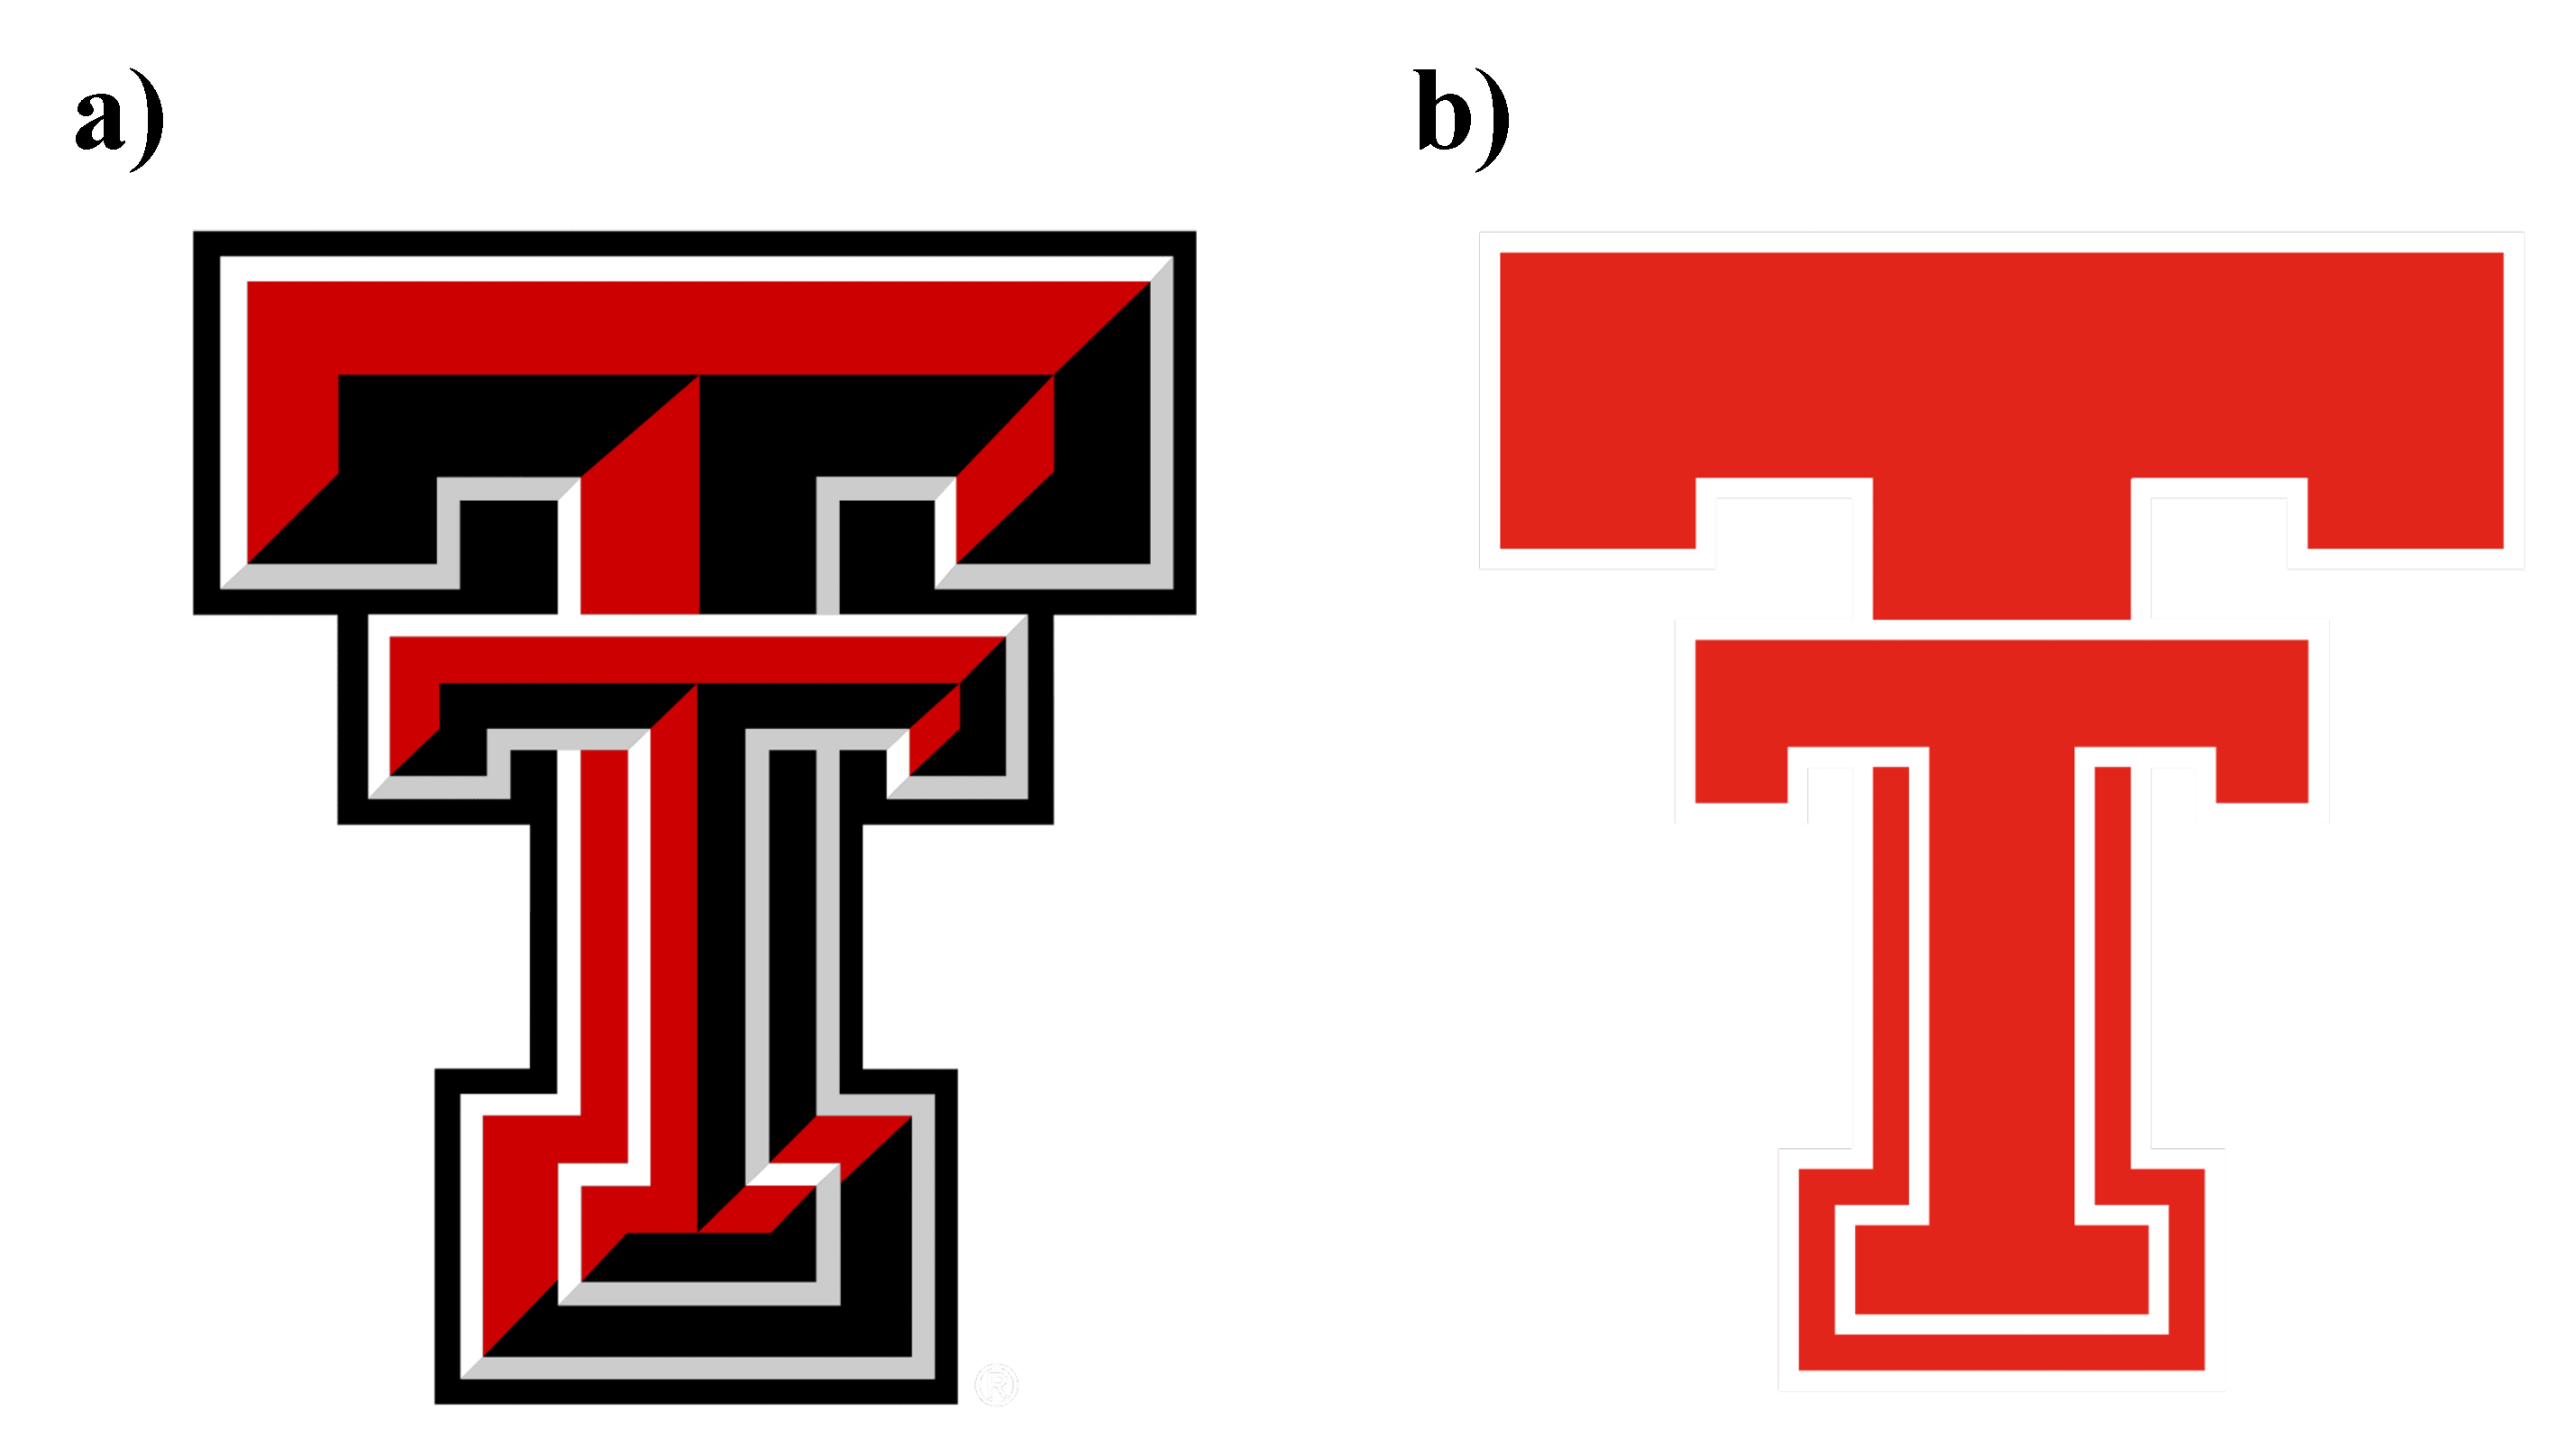
\includegraphics[height=2.2in,
    alt={A comparison of the retro and current Texas Tech University Double-T
    logos}]{figures/example-Double-T.pdf}
  \caption{Comparison of the current (a) and retro (b) Texas Tech University Double-T logos.}
  \label{fig:doublet}
\end{figure}

% HOW TO: a purely decorative image (an ornament, a divider, a logo) gets
% artifact instead of alt. It is then hidden from screen readers, which is
% correct -- it carries no information. Do NOT use artifact on anything a
% reader would need described.
An image that carries no information at all is marked differently. The
ornament below is included with the \verb|artifact| key instead of
\verb|alt|, which removes it from the reading order entirely. The test is
simple: if the image vanished and the reader lost nothing, it is an artifact;
if they lost something, it needs alt text.

\begin{center}
  
\includegraphics[width=2in,artifact]{figures/example-decorative.pdf}
\end{center}

\subsection{Tables}

% HOW TO: a table caption goes ABOVE the table (required), and the table must
% be mentioned in the text before it appears. The first row is tagged
% automatically as the header row.
Table~\ref{tab:example} lists the nominal operating conditions used throughout
this example. Build tables as real tables, never as screenshots: a picture of
a table cannot be read aloud, navigated by column, searched, or corrected. The
first row is tagged as the header row for you, which is what allows a screen
reader to announce a cell as \emph{Pressure, kilopascals: 100} rather than
simply \emph{100}.

\begin{table}
  \caption{Nominal operating conditions for the three test cases.}
  \label{tab:example}
  \begin{tabular}{lrr}
    \toprule
    Case & Pressure (kPa) & Temperature (K) \\
    \midrule
    Low    &  50 &  300 \\
    Medium & 100 &  450 \\
    High   & 200 &  600 \\
    \bottomrule
  \end{tabular}
\end{table}

% HOW TO: a table too long for one page. \endhead repeats the header row on
% every page; \caption[]{...Continued} labels the second and later pages.
% A longtable does not float -- it prints exactly where you put it, so put it
% after the sentence that introduces it.
Table~\ref{tab:example-long} runs past the bottom of the page. A long table
repeats its header row on each new page and is labelled ``Continued'' after
the first, so a reader arriving mid-table still knows what the columns mean.
Long tables do not float: they are set exactly where they appear in the
source, which is why the introducing sentence has to come first.

\begin{longtable}{lrr}
  \caption{Extended parameter sweep spanning more than one page.}
  \label{tab:example-long}\\
  \toprule
  Run & Setting & Result \\
  \midrule
  \endfirsthead
  \caption[]{Continued.}\\
  \toprule
  Run & Setting & Result \\
  \midrule
  \endhead
  \bottomrule
  \endfoot
  R01 & 1.0 & 0.11 \\ R02 & 1.1 & 0.14 \\ R03 & 1.2 & 0.17 \\
  R04 & 1.3 & 0.21 \\ R05 & 1.4 & 0.25 \\ R06 & 1.5 & 0.29 \\
  R07 & 1.6 & 0.34 \\ R08 & 1.7 & 0.39 \\ R09 & 1.8 & 0.44 \\
  R10 & 1.9 & 0.50 \\ R11 & 2.0 & 0.56 \\ R12 & 2.1 & 0.62 \\
  R13 & 2.2 & 0.68 \\ R14 & 2.3 & 0.75 \\ R15 & 2.4 & 0.82 \\
  R16 & 2.5 & 0.89 \\ R17 & 2.6 & 0.96 \\ R18 & 2.7 & 1.04 \\
  R19 & 2.8 & 1.12 \\ R20 & 2.9 & 1.20 \\ R21 & 3.0 & 1.29 \\
  R22 & 3.1 & 1.38 \\ R23 & 3.2 & 1.47 \\ R24 & 3.3 & 1.56 \\
  R25 & 3.4 & 1.66 \\ R26 & 3.5 & 1.76 \\ R27 & 3.6 & 1.86 \\
  R28 & 3.7 & 1.97 \\ R29 & 3.8 & 2.08 \\ R30 & 3.9 & 2.19 \\
  R31 & 4.0 & 2.31 \\ R32 & 4.1 & 2.43 \\ R33 & 4.2 & 2.55 \\
  R34 & 4.3 & 2.67 \\ R35 & 4.4 & 2.80 \\ R36 & 4.5 & 2.93 \\
  R37 & 4.6 & 3.06 \\ R38 & 4.7 & 3.20 \\ R39 & 4.8 & 3.34 \\
  R40 & 4.9 & 3.48 \\ R41 & 5.0 & 3.63 \\ R42 & 5.1 & 3.78 \\
\end{longtable}

\subsection{Equations}

% HOW TO: a numbered display equation with a \label; refer to it with \eqref.
% Screen-reader accessibility is automatic -- the equation is exported as
% MathML, so you do not write alt text for it.
Display equations are numbered at the right margin and are exported as MathML,
which means assistive technology can navigate into a fraction or read a
subscript as a subscript rather than reciting the symbols in a row. No alt
text is written for equations in this template. The saturating behaviour
discussed above is described by

\begin{equation}
  y = \frac{a x}{b + x},
  \label{eq:saturation}
\end{equation}

where $a$ is the asymptotic value and $b$ the half-saturation constant.
Refer to a numbered equation as Equation~\eqref{eq:saturation} rather than as
``the equation above'', which stops being true as soon as a page break moves.

\section{Citations and Links}

% HOW TO: cite with \cite{key}, where key is the name in bibliography/references.bib.
The bibliography is generated from \verb|bibliography/references.bib| by
biber, and citations are numbered in order of first appearance. A reader
struggling to begin the writing itself may take some encouragement from the
concision of earlier contributions to the
literature~\cite{upper1974}, which are inexplicably peer-reviewed. For a more 
conventional demonstration, the method
follows established practice~\cite{example-article} and the underlying theory
is set out in a standard text~\cite{example-book}.

% HOW TO: to print abbreviated journal names instead of full ones, set
% journal-abbreviations = {true} in config/thesis-config.tex. Nothing here
% changes -- the bibliography picks up each entry's shortjournal field.
Journal names print in full by default. Setting
\verb|journal-abbreviations = {true}| in the configuration file switches every
entry that carries a \verb|shortjournal| field to its abbreviated form,
leaving entries without one untouched.

% HOW TO: a web address. Write the address itself so the link text is
% meaningful; bare "click here" links fail the accessibility check.
Link text has to say where it goes. Write the address, or a phrase that
describes the destination; a document whose links all read ``click here'' is
unusable for anyone who navigates by pulling up a list of them. The Graduate
School's requirements are published at
\url{https://www.depts.ttu.edu/gradschool/}.
